\documentclass[a4paper,12pt]{scrartcl}
% \setcounter{secnumdepth}{3}
% \setcounter{tocdepth}{5}

% \makeatletter
% \renewcommand\section{\newpage\@startsection {section}{1}{\z@}%
%                                    {-3.5ex \@plus -1ex \@minus -.2ex}%
%                                    {2.3ex \@plus.2ex}%
%                                    {\normalfont\Large\bfseries}} 
% \renewcommand\paragraph{\@startsection{paragraph}{4}{\z@}%
%                                      {-3.25ex\@plus -1ex \@minus -.2ex}%
%                                      {0.0001pt \@plus .2ex}%
%                                      {\normalfont\normalsize\bfseries}}
% \renewcommand\subparagraph{\@startsection{subparagraph}{5}{\z@}%
%                                      {-3.25ex\@plus -1ex \@minus -.2ex}%
%                                      {0.0001pt \@plus .2ex}%
%                                      {\normalfont\normalsize\bfseries}}
% \makeatother

\newcommand\doctype{Psychologischer Bericht}
\newcommand\supervisor{Prof. Dr. phil. Hugo M. Kehr}
\newcommand\advisor{Dipl. Psych. Stefan Engeser}
\newcommand\deliverydate{4. M{\"a}rz 2011}

\newcommand*{\code}[1]{\texttt{#1}}% style for code insertions

\usepackage[T1]{fontenc}
\usepackage{lmodern}


% \usepackage{pstricks}
% \usepackage{pst-plot}
% \usepackage{auto-pst-pdf}

\usepackage{bibgerm}
\usepackage[hang,flushmargin]{footmisc}
\usepackage[printonlyused]{acronym}
\usepackage{url}
\usepackage[utf8]{inputenc}
\usepackage{graphicx}
\usepackage[hang,small,bf]{caption}
\usepackage{styles/tumlogo}
\usepackage{setspace}
\usepackage[german,english]{babel}
\usepackage{needspace}
\usepackage{fancyhdr}
\pagestyle{fancy}
\headheight 35pt
\lhead{\nouppercase{\leftmark}}
\rhead{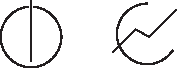
\includegraphics[width=0.5cm]{styles/info.pdf}}


% \selectlanguage{english}

% \usepackage{hyperref} % sorgt f�r f�r Hyperlinks in PDF-Dokumenten
\usepackage[plainpages=false,pdfpagelabels, bookmarks=true]{hyperref}                                             %. hyper-references for ps2pdf 
% \usepackage[ocgcolorlinks]{hyperref}     % sorgt f�r farbige f�r Hyperlinks, die beim Ausdruck schwarz sind
\hypersetup{
    breaklinks=true
    unicode=false,          % non-Latin characters in Acrobat's bookmarks
    pdftoolbar=true,        % show Acrobat's toolbar?
    pdfmenubar=true,        % show Acrobat's menu?
    pdffitwindow=true,      % page fit to window when opened
    pdftitle={},    % title
    pdfauthor={},     % author
    pdfsubject={},   % subject of the document
    pdfnewwindow=true,      % links in new window
    pdfkeywords={}, % list of keywords
    pdfstartview={FitH},
    colorlinks=true,       % false: boxed links; true: colored links
%     linkcolor=red,          % color of internal links
%     citecolor=green,        % color of links to bibliography
%     filecolor=magenta,      % color of file links
%     urlcolor=cyan           % color of external links
    linkcolor=black,          % color of internal links
    citecolor=black,        % color of links to bibliography
    filecolor=black,      % color of file links
    urlcolor=black           % color of external links
}

\makeatletter
\g@addto@macro\UrlBreaks{\do\a\do\b\do\c\do\d\do\e\do\f\do\g\do\h\do\i%
\do\j\do\k\do\l\do\m\do\n\do\o\do\p\do\q\do\r\do\s\do\t\do\u\do\v\do\w%
\do\x\do\y\do\z\do\&\do\1\do\2\do\3\do\4\do\5\do\6\do\7\do\8\do\9\do\0}
%\def\do@url@hyp{\do\-}
\g@addto@macro\UrlSpecials{\do\/{\mbox{\UrlFont/}\hskip 0pt plus 1pt}}
\makeatother

\usepackage{cite}

\widowpenalty=10000
\clubpenalty=10000

\parindent 0pt % keine Absatzeinr�ckung
\parskip 6pt % aber danach ein gewisser Abstand

\graphicspath{{graphics/}}

% \sloppy

%
% der Befehl \hypenation versteht keine Sonderzeichen, also weder ä
% noch "a noch \"a. Wörter die derartige Zeichen enthalten müssen
% direkt im Text getrennt werden, z.B. Wör\-ter
%
\hyphenation{Luft-ma-tra-ze} % in dieses File kommen W�rter die Latex nicht richtig trennt

\begin{document}

\thispagestyle{empty}

\vspace{4cm}
\begin{center}
\oTUM{4cm}\\ 
\vspace{5mm}     
\huge FAKULT{\"A}T F{\"U}R INFORMATIK\\
und\\
FAKULT{\"A}T F{\"U}R WIRTSCHAFTSWISSENSCHAFTEN\\

 
\vspace{0.5cm}
\large DER TECHNISCHEN UNIVERSIT{\"A}T M{\"U}NCHEN\\
\vspace{1mm}
\end{center}

\vspace{10mm}

\begin{center}
\Large \doctype
\vspace{15mm}

\begin{spacing}{1.5}
\huge\bf Flowgame\\%[3ex]
\end{spacing}

\vspace{10mm}
\LARGE Philipp Reichart, Barbara K{\"o}hler,\\ Christopher
H{\"u}bner und Sebastian V{\"o}st

\vspace{10mm}

\begin{figure}[h!]
\centering
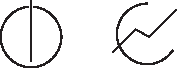
\includegraphics[height=3cm]{styles/info.pdf}
\end{figure}

\end{center}

\thispagestyle{empty}

\vspace{8mm}
\begin{center}
\oTUM{4cm}

\vspace{5mm}     
\huge FAKULT{\"A}T F{\"U}R INFORMATIK\\ 
und\\
FAKULT{\"A}T F{\"U}R WIRTSCHAFTSWISSENSCHAFTEN\\ 
\vspace{0.5cm}
\large DER TECHNISCHEN UNIVERSIT{\"A}T M{\"U}NCHEN\\
\end{center}

\vspace{3mm}

\begin{center}
\Large \doctype
\vspace{2mm}

\begin{spacing}{1.3}
\Huge Flowgame
\vspace{3mm}
\end{spacing}

\begin{tabular}{ll}
\Large Autoren:     & \Large Philipp Reichart, Barbara K{\"o}hler,\\ 
\Large 			  & \Large Christopher H{\"u}bner und Sebastian V{\"o}st\\[2mm]
\Large Aufgabensteller: & \Large \supervisor \\[2mm]				
\Large Betreuer:	   & \Large \advisor    \\[2mm]
\Large Datum:       & \Large \deliverydate
\end{tabular}


\vspace{3mm}

\begin{figure}[hb!]
\centering
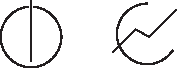
\includegraphics[height=3cm]{styles/info.pdf}
\end{figure}


\end{center}

% \include{disclaimer}
% 
% \pagenumbering{roman}
% \thispagestyle{plain}
% 
% 
% \selectlanguage{english}
% \thispagestyle{plain}
% \begin{abstract}
% \noindent english abstract
% \end{abstract}
% \clearpage

\selectlanguage{german}
% \begin{abstract}
% \noindent Deutsche Kurzfassung
% \end{abstract}
% \clearpage


\tableofcontents
\clearpage

\pagenumbering{arabic}


\clearpage


\section{Einleitung}

\section{Kapitel 2}

\markboth{Abk�rzungsverzeichnis}{Abkürzungsverzeichnis}
\section*{Abk�rzungsverzeichnis}
\addcontentsline{toc}{section}{Abkürzungsverzeichnis}
\begin{acronym}
\acro{DV}{Document Verifier}
\acrodefplural{DV}[DV]{Document Verifiern}
\end{acronym}

\clearpage

\clearpage
\addcontentsline{toc}{section}{Abbildungen}
\listoffigures
  
\clearpage
\addcontentsline{toc}{section}{Literatur}
\bibliography{literatur}{}
\bibliographystyle{alphadin}

\end{document}
